\section{Methods}\label{sec:methods}
This study is quantitative. It compares two harnesses on the same 25 games by their scores, completed levels, actions, and reported tokens. The examples from the runs show how each memory layer worked; they are illustrations, not measurements.

\subsection{Task, information, and scoring}
\subsubsection{Interaction and information}
I evaluated the baseline and layered harnesses on the same versions of 25 public games, containing 183 levels in total. Before each decision, the model received the current board, the numeric identifiers of the actions currently allowed, the game state, the number of completed levels, and selected earlier observations and action records. The controller executed the action specified in the model's reply and could reset the level after a game over. Each reset counted toward the action cap.


The model could not call tools, retrieve information from external sources, inspect game files, or use memory from other games. Prompts contained no game-specific hints. These restrictions applied to the baseline and layered harnesses evaluated here. The historical Tycho study in Appendix~\ref{app:followup} used different restrictions.


\subsubsection{Primary metric (RHAE)}
The primary metric is Relative Human Action Efficiency (RHAE), which combines level completion with action efficiency relative to a human baseline. Higher scores are better. The benchmark scores each game separately and then averages the game scores, giving each game equal weight \citep{arc2026scoring}.

I use $G$ for the number of games, with $G=25$ for both the baseline and layered harnesses. Game $g\in\{1,\ldots,G\}$ contains $L_g$ levels. For level $\ell\in\{1,\ldots,L_g\}$, I set $d_{g\ell}=1$ if the agent completed the level and $d_{g\ell}=0$ otherwise. I use $a_{g\ell}$ for the agent's action count recorded by the scorer and $b_{g\ell}$ for the official human-baseline action count. The level efficiency is
\begin{equation}
q_{g\ell}=\begin{cases}
\min\{1.15,(b_{g\ell}/a_{g\ell})^2\},&d_{g\ell}=1,\\
0,&d_{g\ell}=0.
\end{cases}\label{eq:level}
\end{equation}
An incomplete level contributes a score of zero. For a completed level, efficiency is the squared ratio of the human-baseline action count to the agent's action count, capped at 1.15.

Within each game, level $\ell$ has weight $\ell$, so later levels count more. The total level weight, $W_g$, and the weighted fraction of levels completed, $C_g$, are
\begin{equation}
W_g=\sum_{\ell=1}^{L_g}\ell=\frac{L_g(L_g+1)}{2},\qquad
C_g=\frac{\sum_{\ell=1}^{L_g}\ell d_{g\ell}}{W_g}.\label{eq:completion}
\end{equation}
The percentage game score, $S_g$, uses the weighted mean efficiency but cannot exceed the \emph{completion cap}, $100C_g$. RHAE is the mean of these game scores.
\begin{equation}
S_g=100\min\left\{C_g,\frac{\sum_{\ell=1}^{L_g}\ell q_{g\ell}}{W_g}\right\},\qquad
\operatorname{RHAE}=\frac{1}{G}\sum_{g=1}^{G}S_g.\label{eq:score}
\end{equation}
Efficiency above 1 cannot raise a game's score above its completion cap. Completing every level does not guarantee a score of 100\%. The agent also has to complete the levels efficiently relative to the human action counts.

I recalculated the final baseline and layered-harness scores using the per-level action counts and human baselines stored with the final replay records. The recalculated scores were 46.19821647\% and 85.36898706\%, respectively, reported as 46.20\% and 85.37\%. Appendix~\ref{app:analysis} retains the historical 100-action scoring analysis.

\subsection{Shared baseline and execution process}\label{sec:harness}
Both the baseline and layered harnesses used Claude Opus 5.5 with high effort through the Claude Code command-line interface (CLI), version 2.1.318. They shared the \texttt{hypotheses} stage of \code{research/claude_arc_v1} as their baseline implementation \citep{dai2026code,dai2026layered}. For each decision, the harness started a new CLI session and sent the prompt together with the required JSON response format. I configured the CLI to disable tools, reuse of saved model sessions, project-specific settings, and external connections. To give the model memory between decisions, the harness included the game's saved observations and notes in later requests. The study did not train or fine-tune the model.


The baseline represented each board as rows of hexadecimal color codes and summarized which cells changed between observations. Each request included the current board, up to two earlier full boards, the eight most recent actions, and up to eight hypotheses written by the model. The harness retained these hypotheses across levels and resets within a game, then cleared them before the next game.

Before executing an action, the harness checked that the action was currently allowed, its coordinates were valid, and the reply followed the required JSON structure. If the model cited an earlier board or action result, the harness checked that the reference used an identifier assigned to that record. These checks enforced the required model reply format and reference rules. They did not establish whether the cited evidence supported the model's claim.

Appendix~\ref{app:prompts} reproduces the instructions given to the model (the system prompt) and the required JSON reply structure used in the original 100-action baseline.

\subsection{Memory layers}\label{sec:layers}
The layered harness added four memory layers to the baseline: lessons from game overs or unchanged boards, an object ledger that grouped board regions and stored the model's notes about them, a separate rule list kept across decisions, and a brief for the new level. The baseline included none of these layers.

Table~\ref{tab:feature-configurations} lists the features behind each layer and which of them each configuration enabled. One distinction matters for the controlled tests. The level brief is one layer. The \emph{level-brief package} is the harness setting \texttt{level\_brief}, which enabled the rule list and the brief together with two supporting features. The following sections explain each feature.

\begin{table}[htbp]
\centering\small
\setlength{\tabcolsep}{5pt}
\begin{tabularx}{\linewidth}{@{}Ycccc@{}}\toprule
 & \multicolumn{2}{c}{Whole-game comparison} & \multicolumn{2}{c}{Level-brief tests}\\
\cmidrule(lr){2-3}\cmidrule(l){4-5}
Feature & Baseline & Layered & \shortstack{Without\\package} & \shortstack{With\\package}\\\midrule
\multicolumn{5}{@{}l}{\emph{Baseline evidence}}\\
\quad Current board, up to two earlier boards, eight recent actions, and up to eight hypotheses & Yes & Yes & Yes & Yes\\\addlinespace[3pt]
\multicolumn{5}{@{}l}{\emph{Layer 1: lessons}}\\
\quad Lessons after game overs & No & Yes & Yes & Yes\\
\quad Lessons after no-effect actions & No & Yes & Yes & Yes\\
\quad Model checked actions against lessons & No & Yes & Yes & Yes\\\addlinespace[3pt]
\multicolumn{5}{@{}l}{\emph{Layer 2: object ledger}}\\
\quad Object ledger, notes, and target checks & No & Yes & Yes & Yes\\\midrule
\multicolumn{5}{@{}l}{\emph{Level-brief package: layers 3 and 4, with two supporting features}}\\
\quad Layer 3: separate persistent rule list & No & Yes & No & Yes\\
\quad Layer 4: brief at level transitions & No & Yes & No & Yes\\
\quad Completion feedback: selected frame and changes & No & Yes & No & Yes\\
\quad Flags for newly observed appearance groups & No & Yes & No & Yes\\\bottomrule
\end{tabularx}
\caption{The table lists the features that each configuration enabled. Yes means enabled, with information supplied when applicable. The whole-game comparison switched on every layer at once. The level-brief tests switched only the level-brief package on and off, in both test sets. All four configurations turned off the optional feature for comparing similar board patterns \citep{dai2026layered,dai2026brieftests}.}\label{tab:feature-configurations}
\end{table}

Figure~\ref{fig:harness} shows how the controller prepared the model's input, checked the reply format and whether the selected action was allowed, and executed an accepted action \citep{dai2026layered}. Figures~\ref{fig:lesson-game-over}--\ref{fig:level-brief} show examples from the evaluated runs. They illustrate how the layers worked, but do not measure each layer's effect on performance.

\begin{figure}[htbp]
\centering
\begin{tikzpicture}[node distance=8mm and 16mm,box/.style={draw=accent!60,fill=wash,rounded corners=2pt,align=center,text width=6.2cm,minimum height=15mm,font=\small},arr/.style={-{Stealth[length=2mm]},draw=accent,thick}]
\node[box] (evidence) {\textbf{Prepare the model input}\\Current board and recent action records\\Hypotheses, saved lessons and rules,\\object ledger, and level brief};
\node[box,right=of evidence] (model) {\textbf{Choose the next action}\\Claude Opus 5.5, high effort, tools disabled\\Return one action and the required notes};
\node[box,below=of model] (check) {\textbf{Check the reply}\\Validate its structure, action, coordinates,\\and evidence references};
\node[box,below=of evidence] (update) {\textbf{Execute an accepted action}\\Record the result and update observations\\and memory for the next decision};
\draw[arr] (evidence)--(model);
\draw[arr] (model)--(check);
\draw[arr] (check)--node[above,font=\scriptsize]{Accepted}(update);
\draw[arr] (update)--(evidence);
\draw[arr] (check.east) to[bend right=35] node[right,font=\scriptsize,align=left]{If rejected,\\correction\\requested} (model.east);
\end{tikzpicture}
\caption{\textbf{The controller prepared evidence, checked the model's reply, and executed the selected action.} The layered harness included all four memory layers in this loop. The baseline used the same execution process with those layers disabled. The controller returned rejected replies for correction before it executed an action. The controller derived records from observed boards and actions, while the model wrote the rules and lessons. Those statements could be wrong. The harness cleared all memory before the next game.}\label{fig:harness}
\end{figure}


\subsubsection{Lessons from failures and unchanged boards}
After a game over, the controller reset the level and the model wrote a lesson about what happened. The harness stored the lesson separately from the baseline's hypothesis list and included it in every later request within the same game. Figure~\ref{fig:lesson-game-over} shows one lesson, from the game over that prompted it to the next request. A lesson recorded the model’s interpretation of its observations. The harness did not verify whether that interpretation was correct.

\begin{figure}[htbp]
\centering\footnotesize
\begin{minipage}[t]{0.42\linewidth}
\setlength{\zoomw}{0.465\linewidth}%
\textbf{1. What the agent observed}\par\vspace{3pt}
\begin{tabular}{@{}c@{\hspace{0.05\linewidth}}c@{}}
\begin{markedboard}[\zoomw]{lessons-game-over-a.png}
\draw[black,line width=0.7pt] (0,0) rectangle (0.25,0.0625);
\end{markedboard} &
\begin{markedboard}[\zoomw]{lessons-game-over-b.png}
\draw[black,line width=0.7pt] (0,0) rectangle (0.25,0.0625);
\end{markedboard}\\[1pt]
Before action 357 & After it: game over\\[5pt]
% the boxed corner of each board, four times larger: 16 cells wide, 4 cells high
\begin{tikzpicture}
\begin{scope}\clip (0,0) rectangle (\zoomw,0.25\zoomw);
\node[anchor=south west,inner sep=0pt] at (0,0) {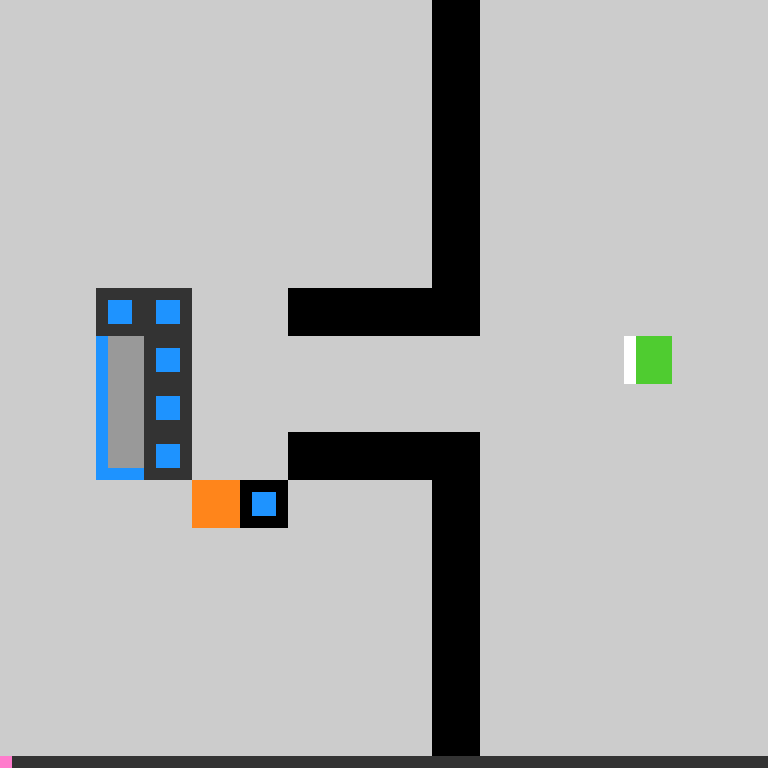
\includegraphics[width=4\zoomw]{figures/runs/lessons-game-over-a.png}};\end{scope}
\draw[black,line width=0.7pt] (0,0) rectangle (\zoomw,0.25\zoomw);
\node[font=\scriptsize,anchor=west,inner sep=1pt] (lab) at (0.2\zoomw,0.16\zoomw) {last pink cell};
\draw[-{Stealth[length=1.6mm]},line width=0.6pt] (lab.west) -- (0.045\zoomw,0.075\zoomw);
\end{tikzpicture} &
\begin{tikzpicture}
\begin{scope}\clip (0,0) rectangle (\zoomw,0.25\zoomw);
\node[anchor=south west,inner sep=0pt] at (0,0) {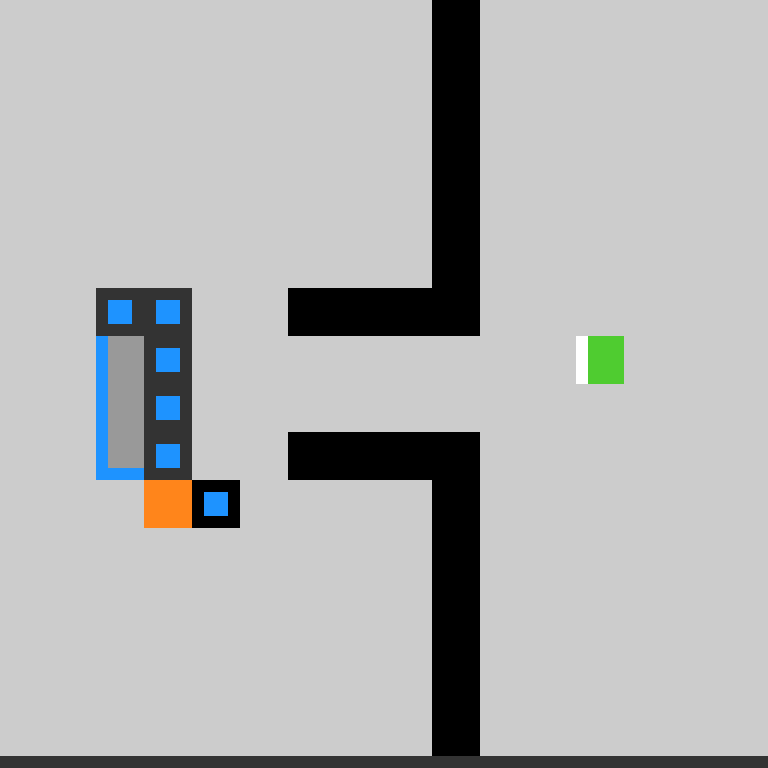
\includegraphics[width=4\zoomw]{figures/runs/lessons-game-over-b.png}};\end{scope}
\draw[black,line width=0.7pt] (0,0) rectangle (\zoomw,0.25\zoomw);
\node[font=\scriptsize,anchor=west,inner sep=1pt] at (0.2\zoomw,0.16\zoomw) {bar empty};
\end{tikzpicture}\\[1pt]
\multicolumn{2}{@{}c@{}}{The boxed corner, four times larger}
\end{tabular}
\end{minipage}\hfill
\begin{minipage}[t]{0.555\linewidth}
\textbf{2. What it stored}, in its reply for action 359\par\vspace{2pt}
\begin{tabularx}{\linewidth}{@{}lY@{}}\toprule
Rule & ``The bar on row 63 is an action budget. Its 7 cells turn to 4 about one every two actions, and the game is over when the last 7 is gone, whatever else is happening on the board.''\\
Applies when & ``Count the 7 cells left on the bottom row and multiply by about 2. If the moves still needed to cover every target tile come to more than that, the attempt will fail. Plan the shortest delivery route from the start and avoid wasted moves.''\\\bottomrule
\end{tabularx}\par\vspace{7pt}
\textbf{3. What the next request showed}, the one for action 360\par\vspace{2pt}
\begin{tabularx}{\linewidth}{@{}lY@{}}\toprule
In the request & The rule and its applies-when clause above, listed under \texttt{game\_over\_lessons} and tagged \texttt{after t357, level 5}\\
The model's check & ``Game-over lesson (budget): 63 of the 64 bottom cells are still 7, so this action will not end the game, and grabbing is needed for the shortest delivery.''\\\bottomrule
\end{tabularx}
\end{minipage}
\caption{\textbf{One game over, the lesson the model wrote from it, and the lesson's return in the next request.} In the layered run of \texttt{wa30}, level 5, action 357 emptied the bar along the bottom row, and the game ended. The controller reset the level, and the model then wrote the lesson in step 2. The harness stored the lesson without checking it and included it in every later request in that game. Step 3 shows the next request and the model's check of its proposed action against the lesson. In the model's text, 7 is the color code of the pink cells and 4 of the dark ones. The model received boards as text; this figure and Figures~\ref{fig:object-ledger} and~\ref{fig:level-brief} draw them in color \citep{dai2026runfigures}. The check in step 3 comes from the run's saved log; the repository records it word for word.}\label{fig:lesson-game-over}
\end{figure}


Some games display a counter or bar that changes as the agent uses actions. The bottom-row bar in Figure~\ref{fig:lesson-game-over} is one, and Figure~\ref{fig:step-counter} in Appendix~\ref{app:no-effect-traces} shows three more. The harness used a heuristic to identify cells belonging to such a counter and excluded them when comparing the boards before and after an action. If no other cells differed, it labeled the action a \emph{no-effect action}. A change in the counter alone therefore did not count as a change to the rest of the board. The class \texttt{CounterMask} in \code{research/claude_arc_v1/recovery.py} of the archived code implements this heuristic \citep{dai2026harnessexport}.

This definition concerns only the compared cells in the final board. Intermediate animation frames could still differ, and game state that was not visible on the board could still change (Figure~\ref{fig:no-effect-examples} in Appendix~\ref{app:no-effect-traces}).

For each no-effect action, the harness kept the action, the board, and a summary of the intermediate frame with the most changed cells relative to the board before the action. The model could write a lesson after taking one additional action and had to write one after taking four additional actions. In later replies, the prompt required the model to check its proposed action against the applicable lessons. These lessons, like those written after game overs, could be wrong.

\Needspace{5\baselineskip}
\subsubsection{Object ledger}
The object ledger recorded detected board regions and the model’s notes about them (Figure~\ref{fig:object-ledger}). The controller identified connected regions, grouped those that looked alike, and recorded where clicks or changes occurred. Each group could contain more than one region on the current board. The model could write notes about a group and select a particular region as the target of its next action. The ledger also marked regions that the agent had not yet clicked and that had not yet changed during recorded play.

The controller detected and grouped regions using fixed rules, which could combine separate objects into a single region or fail to detect relevant objects. The ledger used no object labels or source code provided by the game.

\begin{figure}[htbp]
\centering
\begin{minipage}[c]{0.36\linewidth}
\centering
\begin{markedboard}[\linewidth]{object-ledger-a.png}
\node[note,anchor=west] (aim) at (0.80,0.535) {target on\\this turn};
\draw[pointer] (aim.west) -- (0.762,0.535);
\end{markedboard}
\end{minipage}\hfill
\begin{minipage}[c]{0.60\linewidth}
\footnotesize
\begin{tabularx}{\linewidth}{@{}lrY@{}}\toprule
\shortstack[l]{Appearance\\group} & \shortstack[r]{Detected\\regions} & Model-written note about the group\\\midrule
A & 6 & ``A box. When the player is next to it and facing it, its border turns 3. Action 5 grabs it (border 0). After that, moving toward it pushes it one tile per move. The player can't walk into a box it hasn't grabbed.''\\
AB & 1 & ``An autonomous c block. It moves one tile per player action toward a box, and when it is next to the box it grabs it (the box border turns 4 to 5).''\\
C & 1 & No note yet\\
CY & 1 & No note yet\\
D & 1 & No note yet\\\bottomrule
\end{tabularx}
\end{minipage}
\caption{\textbf{The object ledger grouped regions that looked alike and kept the model's notes about each group across levels.} This example shows \texttt{wa30} at the first decision in level 5, before action 233. Outlines and letters mark the detected regions, and regions with the same letter belong to one appearance group. The table lists the five groups, how many regions each contains, and the notes the model wrote during earlier levels. The arrow marks the region the model chose as its target on this turn: ``I'm aiming at box A at (44,28), the nearest box and right beside the corridor.'' This figure adds the outlines, letters, and arrow; the model received the ledger as text. In the notes, numbers and the letter c are color codes \citep{dai2026runfigures}.}\label{fig:object-ledger}
\end{figure}


\subsubsection{Persistent rules}
The harness kept rules written by the model in a list separate from the baseline's hypotheses and carried the list across decisions within the same game. It held up to 12 rules, each limited to 300 characters. For each rule, the harness stored the level and observation at which it was recorded. When the model replaced a rule, the harness updated the entry with the new rule and its recording information. Once the list was full, the model had to identify an existing rule to replace before adding a new one.

The prompt asked the model to state only what its observations supported and to use less definite wording when the evidence did not support a stronger claim. The harness checked the list size and the identifiers of rules selected for replacement. It did not verify whether the rules were correct.

\subsubsection{Level-transition brief and completion feedback}
Starting with level 2, the model wrote a brief when it entered each level, describing how the previous level ended, what had changed, and what to try next (Figure~\ref{fig:level-brief}).

The brief had four fields. \texttt{won\_by} described how the previous level ended. \texttt{different} described changes in the new level. \texttt{why} gave possible reasons for those changes. \texttt{first} specified the first action to investigate the new level. The harness included the brief in requests throughout the level and allowed the model to correct it.

When the game reported that an action had completed a level, the controller selected an image from that action's animation to help the model understand how the level ended. It excluded the final image, then selected the last remaining image whose dimensions matched the board before the action.

In the next request, the harness showed the selected frame and summarized how its cells differed from the board before the action that completed the level. I call these two items \emph{completion feedback}. If no earlier frame had the required dimensions, the harness reported that it had found no matching frame. Because the selection checked only frame dimensions, the selected frame could already show the next level.

When the object ledger was enabled, the harness flagged groups of board regions whose appearance was not recorded in earlier levels of the same game. A new color or shape did not necessarily mean that a region behaved differently.

The controlled tests compared the package enabled with it disabled, while keeping the object ledger and all other harness settings the same. They measured the package’s combined effect and could not isolate the level brief’s contribution.

\begin{figure}[htbp]
\centering
\begin{minipage}[c]{0.47\linewidth}
\centering
\begin{tabular}{@{}c@{\hspace{6pt}}c@{}}
\begin{markedboard}[0.48\linewidth]{level-brief-a.png}
\node[note,anchor=south west] (won) at (0.04,0.74) {player on the\\last target tile};
\draw[pointer] (0.156,0.74) -- (0.156,0.632);
\end{markedboard} &
\begin{markedboard}[0.48\linewidth]{level-brief-b.png}
\node[note,anchor=north west] (new) at (0.04,0.60) {new block,\\color f};
\draw[pointer] (0.281,0.60) -- (0.281,0.682);
\end{markedboard}\\[1pt]
\footnotesize (a) Completion feedback & \footnotesize (b) First board of level 6
\end{tabular}
\end{minipage}\hfill
\begin{minipage}[c]{0.50\linewidth}
\footnotesize
\begin{tabularx}{\linewidth}{@{}lY@{}}\toprule
Field & What the model wrote (shortened)\\\midrule
\texttt{won\_by} & ``Level 5 completed when the player stepped right onto the last uncovered target tile (8,24). [\ldots] So target tiles covered by the player or by c counted, not only those covered by boxes.''\\
\texttt{different} & ``New things: an f 4x4 block at (16,16). [\ldots] There is no c helper. A wall of 5s, 8 wide, at x44-51, with a gap at rows 24-27.''\\
\texttt{why} & ``Without c, the player has to cover the targets with boxes and/or its own body. The f block is the unknown: maybe a box source, a switch, or a stand-in for a helper.''\\
\texttt{first} & ``Move up toward the f block at (16,16), the new thing, and step next to it to see whether it can be grabbed or reacts.''\\\midrule
Rule added & ``A level completes once every 9-bordered target tile is covered by something: a box, the player, or helper c all count [\ldots].''\\\bottomrule
\end{tabularx}
\end{minipage}
\caption{\textbf{At the start of a new level, the model summarized how the previous level ended and decided what to investigate next.} In the layered run of \texttt{wa30}, action 591 completed level 5. Panel (a) shows the frame the harness selected from that action's animation as completion feedback. Panel (b) shows the first board of level 6. The table quotes the brief the model wrote before its first action in level 6, and the rule it added to its rule list in the same reply. I shortened the quoted text: [\ldots] marks cuts within excerpts, and I also omitted some endings. In the model's text, 5, 9, c, and f are color codes. The brief and the rule are the model's interpretation, which the harness did not check \citep{dai2026runfigures}.}\label{fig:level-brief}
\end{figure}


\subsection{Budgets, validation, and continuation}\label{sec:continuation-design}
I fixed the final cap table on November 18, 2026, before the layered runs began. By then, the baseline had already used 8,402 actions under earlier caps. For 23 of the 25 games, I set the final cap by rounding the whole-game human-baseline action count up to a multiple of 50. For example, the human count of 171 for \texttt{cd82} gave a cap of 200, and the count of 1,843 for \texttt{wa30} gave a cap of 1,850.

Two games kept their earlier caps because the baseline had already won them: \texttt{ft09} kept a cap of 100 despite a human count of 208, and \texttt{sb26} kept a cap of 150 despite a human count of 213. The baseline archive stores the final table. The baseline's later continuations used this table, and each layered run used it from its first action. The caps totaled 17,500 actions across all 25 games for each harness. A run could stop before reaching its game's cap \citep{dai2026continuationfinal}.

The official leaderboard instead gives each level a budget of five times its human-baseline action count and stops the agent once it exhausts that budget \citep{arc2026technical}. I did not enforce this per-level budget during the runs. Section~\ref{sec:result-budget} reports scores recalculated from the recorded action sequences using this budget.

The baseline initially allowed the controller to reset levels up to 10 times across each game. For the baseline continuations, I raised this limit to 50, including for \texttt{tu93}, which had stopped after 10 resets. The layered runs allowed 50 resets per game from the start. Each reset counted toward the game's action cap. The prompts did not tell the model about the reset limit \citep{dai2026continuationfinal}.

For each decision, the controller normally allowed 240 seconds per model call and up to two retries after the initial attempt. For the last 43 recorded actions in \texttt{tr87}, it allowed 400 seconds per call and one retry. The agent completed no additional level during those 43 actions.

Subscription usage limits, slow calls, a lost internet connection, and switches between two subscriptions interrupted some runs. The lost connection stopped \texttt{wa30} at action 1,169. An interrupted run resumed from its saved model replies and game observations, after the runner had checked that it could rebuild every earlier model input exactly. Its earlier actions still counted toward the same cap, so the resumed run was part of the original trial (Appendix~\ref{app:continuation}).

Using the same action caps did not mean that the harnesses made the same number of model calls or sent the same amount of text in each call. The memory layers made model inputs longer, and a rejected reply required another call before the harness could execute a game action. Across the 25 layered runs, the harness rejected 461 of 11,111 replies (4.1\%). Each rejected reply tried to add a rule to the full 12-rule list without identifying an existing rule to replace. Separately, 97 calls exceeded the time limit without returning a reply. Appendix~\ref{app:continuation} gives the full accounting \citep{dai2026logcounts,dai2026wholeverify}.
